%%%%%%%%%%%%%%%%%%%%%%%%%%%%%%%%%%%%%%%%%%%%%%%%%%%%%%%%%%%%%%%%%%%%%%%%%%%%%%%%%%%%%%%%%%%%%%%%%%%%
%                                                                                                  %
%                                              MASTER                                              %
%                                                                                                  %
%%%%%%%%%%%%%%%%%%%%%%%%%%%%%%%%%%%%%%%%%%%%%%%%%%%%%%%%%%%%%%%%%%%%%%%%%%%%%%%%%%%%%%%%%%%%%%%%%%%%


\documentclass{Studienarbeit}

%--------------------------------------------------------------------------------------------------
% REQUIRED PACKAGES
%--------------------------------------------------------------------------------------------------
\usepackage{graphicx} % Include images in the document
\usepackage{appendix} % Appendices at the end of the document.
\usepackage[export]{adjustbox} % adjust and resize boxes/ alignment options for includegraphics
\usepackage{fancyhdr} % Custom header and footer
\usepackage{lastpage} % Reference the number of pages is your document
\usepackage[german]{babel} % Manages culturally-dertermined typographical rules
\usepackage{csquotes} % Advanced facilities for inline and display quotation
\usepackage[nottoc]{tocbibind} % Disables the inclusion of the ToC
\usepackage[hidelinks]{hyperref}% use option [hidelinks] to hide red boxes around links in PDF
\usepackage[
acronym, % acronyms and glossary
automake=immediate, % automake=immediate to be able to print the glossary https://tex.stackexchange.com/questions/468818/glossaries-automake-not-working-lualatex
toc,
section=section,
nopostdot]{glossaries} % create glossary and acronyms
\usepackage[
  backend=biber,
  bibencoding=utf8
]{biblatex} % bibliography


%--------------------------------------------------------------------------------------------------
% DEFINITIONS
%--------------------------------------------------------------------------------------------------
\graphicspath{{figures/}}
\renewcommand{\title}{Titel}
\renewcommand{\author}{Autorname}
\newcommand{\projectname}{Projektname}
\newcommand{\courseofstudies}{Studiengang}
\newcommand{\universityname}{Name der Universität}
\newcommand{\processingperiod}{Bearbeitungszeitraum}
\newcommand{\matnumber}{Matrikelnummer}
\newcommand{\courseabbreviation}{Kursabkürzung}
\newcommand{\companyname}{Firmenname}
\newcommand{\companycity}{Standort der Firma}
\newcommand{\supervisorcompany}{Betreuer der Firma}
\newcommand{\supervisordhbw}{Gutachter der DHBW}
\newcommand{\location}{Ort}


%--------------------------------------------------------------------------------------------------
% PAGE STYLE
%--------------------------------------------------------------------------------------------------
\renewcommand{\floatpagefraction}{.8}

\fancypagestyle{zpagestyle}{ 
\renewcommand{\headrulewidth}{0.5pt}
\renewcommand{\footrulewidth}{0pt}

% delete old header and footer
\fancyhead{}
\fancyfoot{}

% left header
\fancyhead[L]{
\nouppercase{\leftmark}
}

% center header
\fancyhead[C]{
\center
\vspace*{2mm}
}

% right header
\fancyhead[R]{
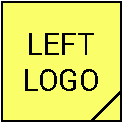
\includegraphics[height=0.8cm]{figures/left_logo.pdf}
\hspace{0.4cm}

\includegraphics[height=0.8cm]{figures/right_logo.pdf}
}
%--------------------------------------------------------------------------------------------------
% left footer
\fancyfoot[L]{
}

% center footer
\fancyfoot[C]{
{\thepage} von \pageref{LastPage}
}

% right footer
\fancyfoot[R]{
}
}
\pagestyle{zpagestyle}%


%--------------------------------------------------------------------------------------------------
% GLOSSARY
%--------------------------------------------------------------------------------------------------
\makeglossaries
\loadglsentries{Glossar}


%--------------------------------------------------------------------------------------------------
% BIBLIOGRAPHY
%--------------------------------------------------------------------------------------------------
\addbibresource{Literatur.bib}

% Break URL in biblatex at lowercase and uppercase characters 
% https://tex.stackexchange.com/questions/134191/line-breaks-of-long-urls-in-biblatex-bibliography
\setcounter{biburllcpenalty}{7000}
\setcounter{biburlucpenalty}{8000}

% Make supercite use square brackets
% From: https://tex.stackexchange.com/a/60923
\DeclareCiteCommand{\supercite}[\mkbibsuperscript]
  {\iffieldundef{prenote}
     {}
     {\BibliographyWarning{Ignoring prenote argument}}%
   \iffieldundef{postnote}
     {}
     {\BibliographyWarning{Ignoring postnote argument}}}
  {\usebibmacro{citeindex}%
   \bibopenbracket\usebibmacro{cite}\bibclosebracket}
  {\supercitedelim}
  {}


%--------------------------------------------------------------------------------------------------
% BEGIN DOCUMENT
%--------------------------------------------------------------------------------------------------
\begin{document}

% TITLEPAGE
\begin{titlepage}
  \newcommand{\HRule}{\rule{\linewidth}{0.5mm}}
  \begin{center}
  \vspace*{-2cm}
  \begin{figure}[!ht]
  \centering
  \begin{minipage}{.5\textwidth}
      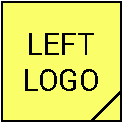
\includegraphics[width=.5\linewidth, left]{figures/left_logo.pdf}
  \end{minipage}%
  \begin{minipage}{.5\textwidth}
      
\includegraphics[width=.5\linewidth, right]{figures/right_logo.pdf}
  \end{minipage}
  \end{figure}
  \vspace*{1cm}
  
  \HRule \\[0.4cm]
  \textsc{\Huge
  \title
  }\\[1mm]
  \HRule \\[1.2cm]
  {\LARGE \projectname} \\[1.2cm]
  \begin{large}
  des Studienganges \courseofstudies \\
  an der \universityname \\[0.5cm]
  von \\
  \author \\[1cm]
  \todayshort \\[1cm]
  \end{large}
  \end{center}
  
  \begin{table}[!ht]
  \begin{large}
  \begin{tabular}{ l l }
      Bearbeitungszeitraum            & {\processingperiod} \\
      Matrikelnummer, Kurs            & {\matnumber}, {\courseabbreviation} \\
      Ausbildungsfirma                & {\companyname}, {\companycity} \\
      Betreuer der Ausbildungsfirma   & {\supervisorcompany} \\
      Gutachter der Dualen Hochschule & {\supervisordhbw}
  \end{tabular}
  \end{large}
  \end{table}
\end{titlepage}

% SPERRVERMERK
\newpage
%%%%%%%%%%%%%%%%%%%%%%%%%%%%%%%%%%%%%%%%%%%%%%%%%%%%%%%%%%%%%%%%%%%%%%%%%%%%%%%%%%%%%%%%%%%%%%%%%%%%
%                                                                                                  %
%                                          BLOCKING NOTICE                                         %
%                                                                                                  %
%%%%%%%%%%%%%%%%%%%%%%%%%%%%%%%%%%%%%%%%%%%%%%%%%%%%%%%%%%%%%%%%%%%%%%%%%%%%%%%%%%%%%%%%%%%%%%%%%%%%

\section*{Sperrvermerk}

Dieser Praxisbericht richtet sich ausschließlich an dessen Gutachter und Mitglieder des Prüfungsausschusses. 
Was zur Folge hat, dass, außer den oben genannten Persönlichkeiten, anderweitigen Personen die Einsicht in diesen Bericht untersagt ist. Ebenfalls ist die Vervielfältigung - auch nur auszugsweise - generell nicht gestattet.


% EIGENSTÄNDIGKEITERKLÄRUNG
%%%%%%%%%%%%%%%%%%%%%%%%%%%%%%%%%%%%%%%%%%%%%%%%%%%%%%%%%%%%%%%%%%%%%%%%%%%%%%%%%%%%%%%%%%%%%%%%%%%%
%                                                                                                  %
%                                     INDEPENDENCE DECLARATION                                     %
%                                                                                                  %
%%%%%%%%%%%%%%%%%%%%%%%%%%%%%%%%%%%%%%%%%%%%%%%%%%%%%%%%%%%%%%%%%%%%%%%%%%%%%%%%%%%%%%%%%%%%%%%%%%%%

% Der Text für die Erklärung wurde aus den Richtlinien für Studienarbeiten der DHBW entnommen:
% https://www.dhbw.de/fileadmin/user_upload/Dokumente/Dokumente_fuer_Studierende/191212_Leitlinien_Praxismodule_Studien_Bachelorarbeiten.pdf
% Stand: Dezember 2019
%
% Der korrekte Ort muss vor der Abgabe/ dem Ausdrucken eingetragen werden.

\section*{Erklärung}

Ich versichere hiermit, dass ich meine {\projectname} mit dem Thema: „{\title}“ selbstständig verfasst und keine anderen als die angegebenen Quellen und Hilfsmittel benutzt habe. Ich versichere zudem, dass die eingereichte elektronische Fassung mit der gedruckten Fassung übereinstimmt.   

\vspace{1cm}

{\location}, den {\todayshort}

\vspace{2.5cm}

\rule{5cm}{0.4pt}

\author

\makeatother

% ABSTRACT
%%%%%%%%%%%%%%%%%%%%%%%%%%%%%%%%%%%%%%%%%%%%%%%%%%%%%%%%%%%%%%%%%%%%%%%%%%%%%%%%%%%%%%%%%%%%%%%%%%%%
%                                                                                                  %
%                                              ABSTRACT                                            %
%                                                                                                  %
%%%%%%%%%%%%%%%%%%%%%%%%%%%%%%%%%%%%%%%%%%%%%%%%%%%%%%%%%%%%%%%%%%%%%%%%%%%%%%%%%%%%%%%%%%%%%%%%%%%%

\section*{Abstract}
\label{sec:abstract}
\addcontentsline{toc}{section}{Abstract}


\section*{Zusammenfassung}
\label{sec:zusammenfassung}
\addcontentsline{toc}{section}{Zusammenfassung}


% INHALTSVERZEICHNIS
\setcounter{tocdepth}{2}
\tableofcontents

% AKRONYME
\clearpage
\printglossary[type=\acronymtype]

% GLOSSAR
\newpage
\printglossary[type=main]

% HAUPTTEIL
%%%%%%%%%%%%%%%%%%%%%%%%%%%%%%%%%%%%%%%%%%%%%%%%%%%%%%%%%%%%%%%%%%%%%%%%%%%%%%%%%%%%%%%%%%%%%%%%%%%%
%                                                                                                  %
%                                             MAIN PART                                            %
%                                                                                                  %
%%%%%%%%%%%%%%%%%%%%%%%%%%%%%%%%%%%%%%%%%%%%%%%%%%%%%%%%%%%%%%%%%%%%%%%%%%%%%%%%%%%%%%%%%%%%%%%%%%%%

\section{Hauptteil}
\label{sec:main}
Text Text Text

% ABBILDUNGSVERZEICHNIS
\listoffigures

% TABELLENVERZEICHNIS
\listoftables

% QUELLCODEVERZEICHNIS
\listoflistings

% LITERATURVERZEICHNIS
\newpage
\printbibliography[heading=bibintoc,title={Literaturverzeichnis}]

% ANHÄNGE
%%%%%%%%%%%%%%%%%%%%%%%%%%%%%%%%%%%%%%%%%%%%%%%%%%%%%%%%%%%%%%%%%%%%%%%%%%%%%%%%%%%%%%%%%%%%%%%%%%%%
%                                                                                                  %
%                                              ANHAENGE                                            %
%                                                                                                  %
%%%%%%%%%%%%%%%%%%%%%%%%%%%%%%%%%%%%%%%%%%%%%%%%%%%%%%%%%%%%%%%%%%%%%%%%%%%%%%%%%%%%%%%%%%%%%%%%%%%%


\begin{appendices}
\section*{Anhänge}
\addcontentsline{toc}{section}{Anhänge}
\markboth{Anhänge}{Anhänge}
\renewcommand{\thesubsection}{\Alph{subsection}}

\subsection{Anhang 1}
\label{appx:appendix1}

Here is an appendix.

\end{appendices}

\end{document}